\subsection{Measuring SWR: What's Your Tool?}

\begin{tcolorbox}[colback=gray!10, colframe=black, title=E4A08]
Which of the following is used to measure SWR?
\begin{enumerate}[label=\Alph*.]
    \item Directional wattmeter
    \item Vector network analyzer
    \item Antenna analyzer
    \item \textbf{All these choices are correct}
\end{enumerate} \end{tcolorbox}

To understand the question above, we need to grasp the concept of Standing Wave Ratio (SWR) and the tools that can be employed to measure it. SWR is a critical parameter in radio communication that indicates how well the antenna is matched to the transmission line. An SWR of 1:1 signifies perfect matching, while values greater than 1:1 indicate increasing mismatches.

There are multiple instruments that can be used to measure SWR:

1. \textbf{Directional wattmeter}: This device measures forward and reflected power. The SWR can be calculated using the formula:
   \[
   SWR = \frac{P_f + P_r}{P_f - P_r}
   \]
   where \(P_f\) is the forward power and \(P_r\) is the reflected power.

2. \textbf{Vector network analyzer (VNA)}: While primarily used for measuring the S-parameters of a device under test (DUT), a VNA can also be utilized to derive SWR from the reflection coefficient.

3. \textbf{Antenna analyzer}: This device directly measures SWR and is specifically designed for testing antennas.

Given the definitions above, 

In order to visualize the concept of SWR, we may consider the diagram below, which illustrates the relationship between the forward and reflected waves in a transmission line.

\begin{center}
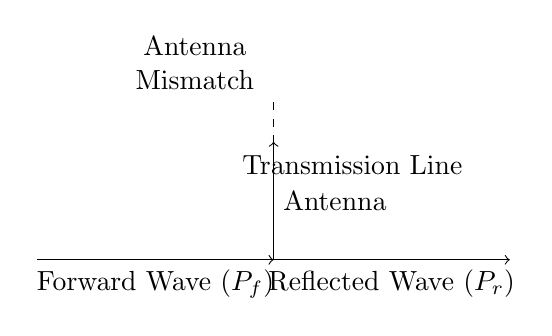
\begin{tikzpicture}
    \draw[->] (0,0) -- (3,0) node[midway, below] {Forward Wave ($P_f$)};
    \draw[->] (3,0) -- (3,1.5) node[midway, right] {Antenna};
    \draw[->] (3,0) -- (6,0) node[midway, below] {Reflected Wave ($P_r$)};
    \draw[dashed] (3,0) -- (3,2);
    \node at (4, 1.2) {Transmission Line};
    \node[align=center] at (2, 2.5) {Antenna \\ Mismatch};
\end{tikzpicture}
\end{center}
